\documentclass[twocolumn]{revtex4-1}
\usepackage{graphicx}
\usepackage{float}
\usepackage[breaklinks, colorlinks, citecolor=blue]{hyperref}
\usepackage{natbib,hyperref,ifthen}
\bibliographystyle{arxiv}

\newcommand{\comment}[1]{{\color{red}#1}}

\begin{document}

\title{The problem with calculating tensions}
\author{Tom Charnock}
\email{tom.charnock@nottingham.ac.uk}
\affiliation{Centre for Astronomy \& Particle Theory, University of Nottingham, University Park, Nottingham, NG7 2RD, U.K.}
\maketitle

    Calculating the similarity between two different distributions is notoriously difficult.
    The main problem is robustness over a wide variety of different situations.
    For example, if two distributions have the same mean, but the variance of one is greater than the other, the agreement should be high.
    Most quantifications would show that their similarity is low.
    The Bhattacharyya distance is one example where this problem arises.
    It is defined as 
    \begin{equation}
        BC(P_1, P_2) = \int dx \sqrt{P_1(x)P_2(x)}.
    \end{equation}
    Take two normal distributions, $P_1(x)$ and $P_2(x)$.
    Shown in Fig.~\ref{fig:bhattacharrya} are three cases, the first where $P_1(x) = P_2(x)$, the second where the means of $P_1(x)$ and $P_2(x)$ are equal but the standard deviation of $P_2(x)$ is larger and finally where the means of $P_1(x)$ and $P_2(x)$ are different (with the same standard deviation) such that the distributions do not overlap.
    \begin{figure}
        \centering
        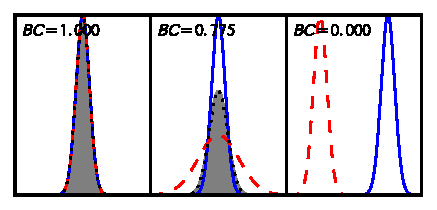
\includegraphics{../comparison/plots/Bhattacharrya.pdf}
        \caption{Values of the Bhattacharrya distance for three different distributions.
                 The blue and red-dashed curves are the probability distribution functions $P_1(x)$ and $P_2(x)$ respectively.
                 The shaded area (bounded by a black-dotted line) is the integrated region for the Bhattacharrya distance.}
        \label{fig:bhattacharrya}
    \end{figure}
    \noindent The blue curve indicates the values of $P_1(x)$ and $P_2(x)$ is depicted by the red dashed curve.
    It is clear that the distributions in the first subplot are in complete agreement.
    The black-dotted line shows the integrated quantity $\sqrt{P_1(x)P_2(x)}$, with the shaded region being the area under the integrated curve.
    The Bhattacharyya distance for this is $BC = 1$.
    The middle panel shows that $P_1(x)$ is in complete agreement within $P_2(x)$ although some values of $P_2(x)$ would fall outside of $P_1(x)$.
    The Bhattacharyya distance in this case (when the standard deviation of $P_2(x)$ is three times that of $P_1(x)$) is $BC = 0.775$. 
    The last subplot is completely disparate and has $BC = 0$.
    The first and last $BC$ values are understandable.
    The problem here is in the second subplot.
    Quoting one number to state the agreement between two distributions, rather than stating in how much agreement one is with another causes some misunderstanding.
    This is clearly an issue when quantifying tension.
    There is some degeneracy between the widening of distributions and shifting of means keeping the width of the distribution the same.
    This can be seen in Fig.~\ref{fig:bhattacharrya_2}.
    \begin{figure}
        \centering
        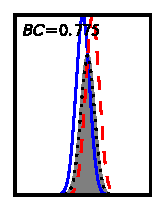
\includegraphics{../comparison/plots/Bhattacharrya_2.pdf}
        \caption{Shifting the means of one of the probability distributions instead of making the distribution wider gives the same $BC$ as the middle panel of Fig.~\ref{fig:bhattacharrya}.}
        \label{fig:bhattacharrya_2}
    \end{figure}
    \noindent The Bhattacharrya distance is therefore not quite illuminating the true agreement between the distributions.
    In the middle panel of the Fig.~\ref{fig:bhattacharrya} all of $P_1(x)$ is in agreement with $P_2(x)$ even though $P_2(x)$ will contain samples outside of $P_1(x)$.
    In Fig.~\ref{fig:bhattacharrya_2}, however, there are both samples in $P_1(x)$ which are not in $P_2(x)$ an vice versa.
    \\
    \\
    Another option is to calculate the overlap coefficient.
    This is given by the integral under the minimum of the two distributions
    \begin{equation}
        OVL = \int dx~{\rm Min}[P_1(x), P_2(x)].
    \end{equation}
    In a similar way to the Bhattacharrya distance this gives one value to quantify similarity and punishes comparisons of distributions where one distribution is wider than the other.
    This can be seen in Fig.~\ref{fig:overlap}.
    \begin{figure}
        \centering
        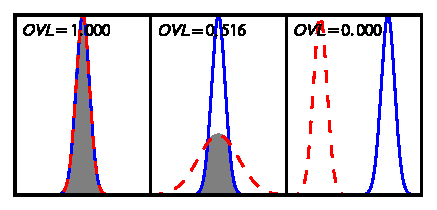
\includegraphics{../comparison/plots/overlap.pdf}
        \caption{Values of the overlap coefficient for the same distributions as in Fig.~\ref{fig:bhattacharrya}. The shaded regions are the integrated quantities.}
        \label{fig:overlap}
    \end{figure}
    \noindent The shaded area is integrated over.
    The first and last panels (left to right) again give answers which are understandable, but the middle subplot now suggests that the agreement is lower than the Bhattacharrya distance.
    Again the widening of the distribution is equivalent to a shift in the means in a similar way to Fig.~\ref{fig:bhattacharrya_2}.
    This can be seen in Fig.~\ref{fig:overlap_2}.
    \begin{figure}
        \centering
        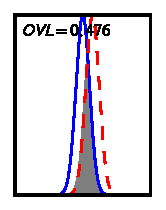
\includegraphics{../comparison/plots/overlap_2.pdf}
        \caption{Shifting the means of the probability distribution instead of making the distribution wider gives a lower $OVL$ than the middle panel of Fig.~\ref{fig:overlap}.}
        \label{fig:overlap_2}
    \end{figure}
    \noindent The $OVL$ for the shift in means is less than that due to the widening of the distribution and so more distant ($P_1(x)$ mean to $P_2(x)$ mean) is quantified as more different than the completely overlapping distributions.
    Care needs to be taken in interpreting the Bhattacharrya distance and the overlapping coefficient since they are on different scales. 
    For the same change in means, the value of $BC$ is higher than $OVL$. 
    These numbers are somewhat arbitrary and don't relate to a statistical significance of any sort.
    \\
    \\
    In \cite{Battye:2014qga} a slightly different tack was taken.
    Here the distributions are first combined as a difference vector
    \begin{equation}
        {\bf P}(y) = x^{P_1}_i-x^{P_2}_j~\forall~i,j,
    \end{equation}
    where $y=x_i-x_j$ with $x^{P_a}_i$ being the $i^{\rm th}$ $x$ value from the distribution $P_a$.
    The value of the probability distribution function at zero gives an indication how similar the two original distributions are.
    To quantify this similarity the integral of the probability distribution greater than the value of the probability distribution function at zero needs to be found
    \begin{equation}
        C = \oint_{{\bf P}(0)} dy{\bf P}(y).
    \end{equation}
    Integrating areas under (or within) the probability distribution allows the result to be directly related to statistical significances.
    In fact, in \cite{Battye:2014qga} this statistical significance is mapped onto the number of standard deviations of a one dimensional Gaussian, i.e $C=0.68$ gives a tension of $\sim1\sigma$.
    This method removes the problem with underestimating the similarity of distributions with different widths as can be seen in Fig.~\ref{fig:charnock}.
    \begin{figure}
        \centering
        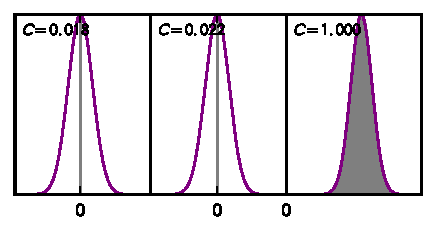
\includegraphics{../comparison/plots/Charnock.pdf}
        \caption{Combined difference vector formed from the same distributions as in Figs.~\ref{fig:bhattacharrya} and~\ref{fig:overlap}. The shaded area shows the integrated region of the distribution about the probability distribution function value at zero.}
        \label{fig:charnock}
    \end{figure}
    \noindent The first and second subplots are both completely in agreement with each other.
    In the case of the second panel, the distribution is now wider but consistent and so has a value of $C \approx 0$, i.e. there is no tension $\sim0\sigma$.
    Since the value of the probability distribution function at zero in the third subplot is essentially zero then the integral about the zero isocontour is $C\approx1$ and the agreement is only correct at an extremely large number of standard deviations, i.e. there is a lot of tension.
    At first appearances this seems to solve the problem somewhat, but information has been lost about the width of initial distributions.
    It is a matter of opinion whether this is necessary information or not.
    The value of $C\gtrsim0$ in the first panel of Fig.~\ref{fig:charnock} since a finite number of samples from the distributions were taken to form the difference vector.
    $C=0$ would be obtained with in the limit of infinite numbers of samples.
    When the mean of $P_2(x)$ is shifted, as in Figs.~\ref{fig:bhattacharrya} and~\ref{fig:overlap_2}, the value of $C=0.685$ which shows that the distributions disagree at a greater extent than the middle panel of Fig.~\ref{fig:charnock}.
    This can be seen in Fig.~\ref{fig:charnock_2}.
        \begin{figure}
        \centering
        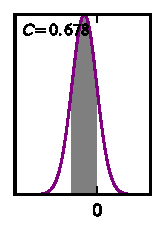
\includegraphics{../comparison/plots/Charnock_2.pdf}
        \caption{The equivalent of Fig.~\ref{fig:overlap_2} using the method of \cite{Battye:2014qga}. The shaded regions are integrated to give $C$.}
        \label{fig:charnock_2}
    \end{figure}
    \noindent The tension in the middle panel of Fig.~\ref{fig:charnock} is essentially zero whilst it is $\sim1\sigma$ in Fig.~\ref{fig:charnock_2}.
    This seems a sensible answer as the mean of the distribution has shifted approximately one standard deviation (actually slightly more, the shift in the mean was chosen such that the $BC$ value in the middle panel of Fig.~\ref{fig:bhattacharrya} was equal to $BC$ in Fig.~\ref{fig:bhattacharrya_2}).
    Another problem with this method is interpreting what the integral of the values above the probability distribution function at $y=0$ means.
    A more useful description perhaps would be to integrate the probability distribution function above and below $y=0$ and use these two numbers as some quantification.
    This becomes less desirable in higher dimensions where there are two numbers per dimension to considered.
    The quantity $C$, then, gives a good indication of the level of tension in one number independent of the number of dimensions considered.
    \\
    \\
    Each of these methods so far discussed can deal with non-Gaussian distributions, but whether they give a good description of the amount of agreement is again another matter.
    \begin{figure}
        \centering
        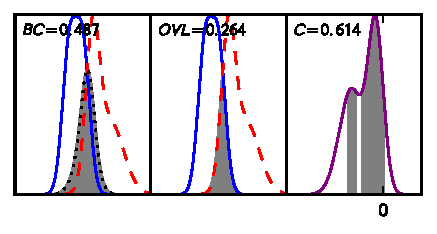
\includegraphics{../comparison/plots/skew.pdf}
        \caption{Non-Gaussian distributions for each of the previous methods, $BC$, $OVL$ and $C$.
                 The blue and red-dashed curves indicate the probability distributions $P_1(x)$ and $P_2(x)$ respectively, whilst the purple curve in the third panel depicts the value of the probability distribution of the difference vector.
                 The shaded region is integrated to get the tension quantification.}
        \label{fig:skew}
    \end{figure}
    \noindent The middle panel of Fig.~\ref{fig:skew} shows two non-Gaussian distributions which partially overlap.
    How to interpret each of the measures in this case is difficult.
    When $BC = 0.487$ or $OVL=0.264$ it is seen that the agreement between the two distributions is less than a shift in the means of approximately one standard deviation, or likewise, less agreement than a widening of one of the distributions by a factor of two.
    This highlights one way to interpret the values of $BC$ and $OVL$.
    $BC=0.487$ is equivalent to a shift in one of the means of two identical distributions by $\sim2.4\sigma$.
    $OVL=0.264$ is equivalent to a shift in one of the means of two identical distributions by $\sim2.3\sigma$.
    It is useful that these two values agree to some extent in what the shifts can be interpreted as, although, the main problem in that wide distributions still cause disagreement still persists.
    On the other hand, $C$ can still be interpreted easily as a statistical significance equivalent to $\sim0.85\sigma$.
    The problem here is that the $C$ method appears to be in a lot less tension than $BC$ or $OVL$ would suggest.
    Of course, since the width of the distribution isn't taken into account then $C$ should give less tension than the other two methods, but in this non-Gaussian should this be the case?
    \\
    \\
    A fourth option for quantifying tensions is to throw away the single number method and state how much tension there is between one distribution and the other and also the reverse.
    One efficient way to do this is to calculate the integral of $P_1(x)$ within a given set of limits of $P_2(x)$.
    For example to find out the percentage of samples from $P_1(x)$ are within, say, the 3$\sigma$ values of $P_2(x)$.
    \begin{eqnarray}
        I_1 & = \displaystyle\int_{P_2(3\sigma)}dx P_1(x),\\
        I_2 & = \displaystyle\int_{P_1(3\sigma)}dx P_2(x).
    \end{eqnarray}
    An example can be seen in Fig.~\ref{fig:under}.
    \begin{figure}
        \centering
        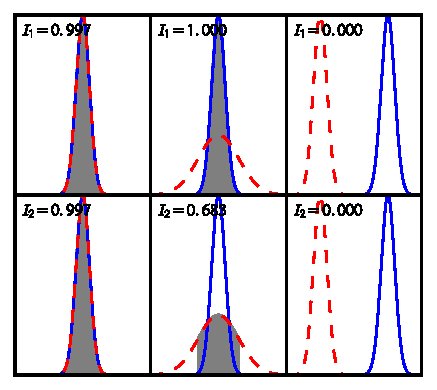
\includegraphics{../comparison/plots/under.pdf}
        \caption{The amount of agreement for each distribution compared to the other. 
                 The top row shows the amount of $P_1(x)$ within the 3$\sigma$ limits of $P_2(x)$ and the bottom row shows the amount of $P_2(x)$ within the 3$\sigma$ limits of $P_1(x)$. 
                 The shaded area is the 3$\sigma$ integrated region.}
        \label{fig:under}
    \end{figure}  
    \noindent It is very easy to see how much of one distribution fits within the other using this technique.
    For example, when the two distributions are equal then the statistical significances at the 3$\sigma$ level should be equal (as in the first column of Fig.~\ref{fig:under}) and equivalent to the integral under a normal distribution between the 3$\sigma$ interval, i.e. $I\approx0.997$.
    The second column of Fig.~\ref{fig:under} shows that the whole distribution of $P_1(x)$ is within the 3$\sigma$ interval of $P_2(x)$ but only 68.2\% of the samples from $P_2(x)$ fit within the 3$\sigma$ interval of $P_1(x)$.
    As expected, the third column shows there is no agreement between the two distributions.
    Fig.~\ref{fig:under_2} shows how shifting one of the means of two identical distributions changes the limits of integration for the other distribution.
    This provides a fairly robust method of quantifying the difference between two distributions but does depend on setting arbitrary limits and knowing the distributions well to a large number of standard deviations.
    Although there are two numbers (or more if calculating the integrals between more limits, i.e. 1, 2, 3, ... $\sigma$ intervals) they should be considered together to give a true understanding of the agreement.
    Taking either of the numbers in the first column of Fig.~\ref{fig:under} individually would possibly suggest that the data isn't in exact agreement, which it is.
    The ratio though gives the indication that the distributions are identical and using the fact that the $3\sigma$ limits contains 99.7\% of the samples reveals that distributions are indeed the same.
    The middle column of Fig.~\ref{fig:under} shows how a widening of the distribution (keeping the mean the same) just changes the ratio of the number of samples within each of the distributions.
    This allows the statement of agreement of one distribution to the other to be discussed.
    In this example, all of $P_1(x)$ is contained within the 3$\sigma$ interval of $P_2(x)$ and is therefore in \emph{complete agreement within 3$\sigma$}.
    By reducing the $P_2(x)$ limits to 1 or 2$\sigma$ then even tighter constraints on the agreement of $P_1(x)$ to $P_2(x)$ can be stated.
    It makes less sense in this case to state the agreement of $P_2(x)$ in comparison to $P_1(x)$.
    The tension here is not due to disagreement in the results, only due to uncertainty.
    This is a somewhat useful quantity in itself.
    In this case there is certainty that \emph{1$\sigma$ of $P_2(x)$ is within the 3$\sigma$ interval of $P_1(x)$}.
    \begin{figure}
        \centering
        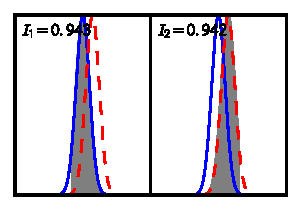
\includegraphics{../comparison/plots/under_2.pdf}
        \caption{Equivalent of Figs.~\ref{fig:bhattacharrya_2},~\ref{fig:overlap_2} and~\ref{fig:charnock_2} using the method in Fig.~\ref{fig:under}.}
        \label{fig:under_2}
    \end{figure}
    \noindent In Fig.~\ref{fig:under_2} the distributions are the same but the mean of one distribution is shifted.
    The ratio of one to the other shows that the distributions are similar in shape, but the fact that the percentage of samples within the $3\sigma$ interval is less than 99.7\% shows that the means have been shifted.
    The more disparate the distributions the fewer the number of samples in the integral limits.
    \begin{figure}
        \centering
        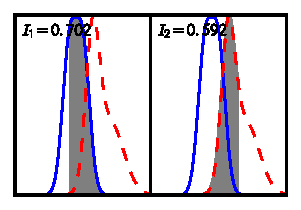
\includegraphics{../comparison/plots/under_skew.pdf}
        \caption{Equivalent of Fig.~\ref{fig:skew} using the method in Fig.~\ref{fig:under}.}
        \label{fig:under_skew}
    \end{figure}
    \noindent For distributions where there are shifts in the mean and a widening of distributions or are non-Gaussian, as in Fig.~\ref{fig:under_skew}, similar assumptions can be made.
    The larger number from the distribution fits better, i.e. has a more peaky distribution than the distribution which has a smaller number.
    Comparing the larger number to the value of integrating equal distributions between the $3\sigma$ intervals gives the amount of agreement, i.e. shows the shift in the means.
    In the case of non-Gaussian distributions there is more information than just the shift in the means and the widening of distributions which is not as easily quantified with just the two numbers.
    Fortunately there is still the general trend with similar values for both distributions showing similar shaped distributions and lower values showing greater tension.
    \\
    \\
    So far, all of these methods have been discussed in only one dimension.
    They can all be generalised to multiple dimensions.
    For example the equivalent plots to Figs.~\ref{fig:bhattacharrya},~\ref{fig:overlap},~\ref{fig:charnock} and~\ref{fig:under} in two dimensions can be found in Fig.~\ref{fig:2D}.
    \begin{figure}
        \centering
        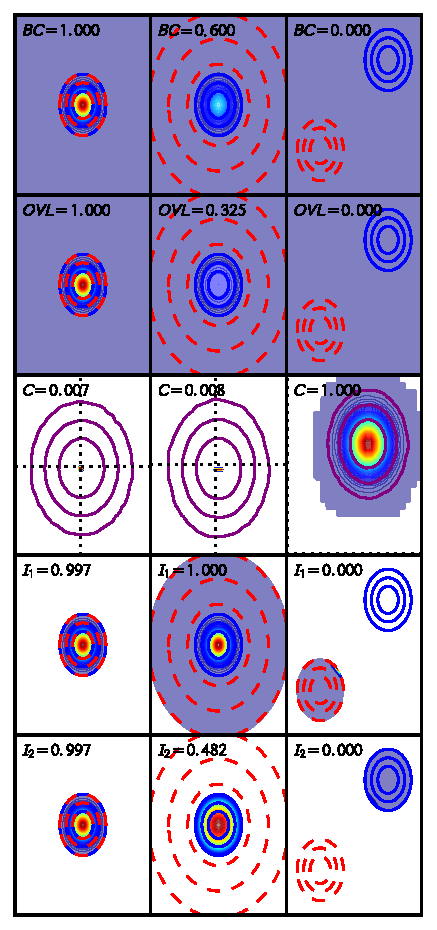
\includegraphics{../comparison/plots/2D.pdf}
        \caption{The top three rows are the equivalent of Figs.~\ref{fig:bhattacharrya},~\ref{fig:overlap} and~\ref{fig:charnock} in two dimensions.
                 The last two rows are the equivalent of Fig.~\ref{fig:under} in two dimensions.
                 In each case the shaded area is integrated, redder areas being larger probability distribution function values and bluer areas being smaller.
                 The blue and red-dashed contours in the first, second, fourth and fifth rows are the 1, 2 and 3$\sigma$ contours for $P_1({\bf x})$ and $P_2({\bf x})$ respectively.
                 The purple contours in the third row are the 1, 2 and 3$\sigma$ contours for the difference vector.}
        \label{fig:2D}
    \end{figure}
    In the first column the two distributions $P_1({\bf x})$ and $P_2({\bf x})$ are identical.
    In the second column the width of the distribution $P_2({\bf x})$ is three times as wide in both dimensions as $P_1({\bf x})$ with identical means.
    In the final column the two distributions are very distinct from each other.
    In the first, second, fourth and fifth rows the blue and red-dashed lines refer to the 1, 2 and 3$\sigma$ contours for $P_1({\bf x})$ and $P_2({\bf x})$ respectively.
    The shaded area in all subplots is integrated over to get each statistical measure.
    Redder regions have a larger probability distribution function value, and bluer areas have lower values.
    The top two rows show similar results to each other, which follow the same trend as the results from Figs.~\ref{fig:bhattacharrya} and~\ref{fig:overlap}.
    The two identical distributions give $BC = 1$ and $OVL = 1$ as expected.
    Comparing a diffuse distribution to a peakier distribution (as in the second column) also gives similar values to those in Figs.~\ref{fig:bhattacharrya} and~\ref{fig:overlap}.
    $BC$ and $OVL$ are lower in this case since the distributions also ``disagree'' more (in the other dimension).
    Finally the last column gives exactly the expected results.
    The third row is the equivalent to Fig.~\ref{fig:charnock}.
    The purple lines show the 1, 2 and 3$\sigma$ contours and the shaded region is integrate.
    The integrated region is formed from the probability distribution above the distribution at ${\bf y} = 0$.
    The first two columns show that the difference vector is a two dimensional normal distributions centred on ${\bf y}=0$ with the shaded region being integrated to give the slight non-zero values for $C$, which is due to using a finite number of samples.
    The last column shows that the difference vector is well away from zero in both dimensions.
    Since the distribution is so far from zero the value of the probability distribution function is essentially zero, so does not contribute the integral.
    This region is white in the subplot.
    The last two rows are the equivalent of Fig.~\ref{fig:under}.
    The shaded regions show that the integration only takes place within the 3$\sigma$ contours of the comparison distribution.
    The results again follow the outcome from the one dimensional case.
    \\
    \\ 
    The equivalent plot to Figs.~\ref{fig:bhattacharrya_2},~\ref{fig:overlap_2} and~\ref{fig:charnock_2} in two dimensions can be found in Fig.~\ref{fig:2D_2}.
    When shifting one of the means of two identical distributions the values of $BC$ and $OVL$ are similar to keeping the means the same, but widening one distribution.
    On the other hand, the integral under the curve in the third panel is approximately one standard deviation difference when shifting the mean rather than no difference when just widening the distribution, as in Fig.~\ref{fig:charnock_2}.
    \begin{figure}
        \centering
        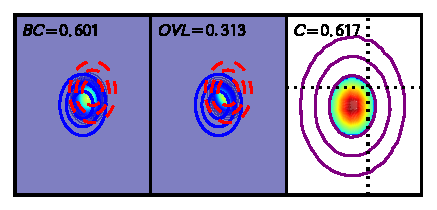
\includegraphics{../comparison/plots/2D_2.pdf}
        \caption{The three columns are the equivalent of Figs.~\ref{fig:bhattacharrya_2},~\ref{fig:overlap_2} and~\ref{fig:charnock_2} in two dimensions.
                 In each case the shaded area is integrated, redder areas being larger probability distribution function values and bluer areas being smaller.
                 The blue contours in the first two columns are the $P_1({\bf x})$ 1, 2 and 3$\sigma$ contours and are red-dashed for $P_2({\bf x})$.
                 The purple contours in the third column are the 1, 2 and 3$\sigma$ contours for the difference vector ${\bf P}({\bf y})$.}
        \label{fig:2D_2}
    \end{figure} 
    \noindent The equivalent plot to Fig.~\ref{fig:under_2} in two dimensions can be found in Fig.~\ref{fig:under_2D}.
    Again it can be seen that the integrated areas are contained within the 3$\sigma$ contour lines of the comparison distribution.
    Since $I_1 = I_2$ the distributions are equivalent in shape, but as they are less than $\sim0.997$ then the mean has been shifted, indicating some tension.
    \begin{figure}
        \centering
        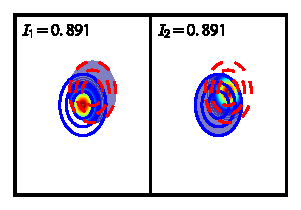
\includegraphics{../comparison/plots/under_2D.pdf}
        \caption{The equivalent of Fig.~\ref{fig:under_2} in two dimensions.
                 The shaded area is integrated, redder areas being larger probability distribution function values and bluer areas being smaller.
                 The blue and red-dashed contours are the 1, 2 and 3$\sigma$ contours for $P_1({\bf x})$ and $P_2({\bf x})$ respectively.}
        \label{fig:under_2D}
    \end{figure} 
    \noindent The equivalent plot to Fig.~\ref{fig:skew} in two dimensions can be found in Fig.~\ref{fig:skew_2D}.
    The first two columns show that, even though the majority of the ``peakier'' distribution overlap, there is little agreement between the distributions due to the way they are combined.
    On the other hand, the third column shows that the difference vector is actually quite close to zero.
    It looks like a lot of the samples are quite far from zero here.
    This is where integrating only above the value of the probability distribution function at zero may become contentious.
    Using this measure does, at least, show that there is a good agreement with most of the distribution, or the most likely part of the distribution.
    It is only the outlying samples which cause some uncertainty, and this is not quantified by the $C$ measure.
    \begin{figure}
        \centering
        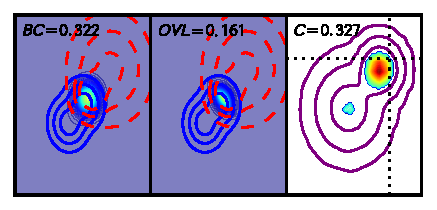
\includegraphics{../comparison/plots/skew_2D.pdf}
        \caption{The three columns are the equivalent of the three columns in Fig.~\ref{fig:skew} in two dimensions.
                 In each case the shaded area is integrated, redder areas being larger probability distribution function values and bluer areas being smaller.
                 The blue contours in the first two columns are the $P_1({\bf x})$ 1, 2 and 3$\sigma$ contours and are red-dashed for $P_2({\bf x})$.
                 The purple contours in the third column are the 1, 2 and 3$\sigma$ contours for the difference vector ${\bf P}({\bf y})$.}
        \label{fig:skew_2D}
    \end{figure}
    \noindent Finally, the equivalent plot to Fig.~\ref{fig:under_skew} in two dimensions can be found in Fig.~\ref{fig:under_skew_2D}.
    \begin{figure}
        \centering
        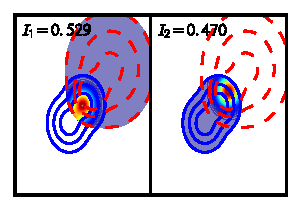
\includegraphics{../comparison/plots/under_skew_2D.pdf}
        \caption{The equivalent of Fig.~\ref{fig:under_skew} in two dimensions.
                 The shaded area is integrated, redder areas being larger probability distribution function values and bluer areas being smaller.
                 The blue and red-dashed contours are the 1, 2 and 3$\sigma$ contours for $P_1({\bf x})$ and $P_2({\bf x})$ respectively.}
        \label{fig:under_skew_2D}
    \end{figure}
    \noindent This result can be interpreted exactly as before.
    Both distributions are fairly similar in distribution size (due to $P_1({\bf x})$ being peakier but with two fairly distinct maxima, whilst $P_2({\bf x})$ is wider but with only one maxima).
    This means that that values of $I_1$ and $I_2$ are quite close.
    The more interesting information comes from the fact that $I_1$ or $I_2$ are both considerably less than $\sim0.977$ and are therefore quite disparate.
    \\
    \\
    It is now difficult to quantify the difference between the distributions and, in fact, becomes a matter of preference.
    In two dimensions it can be seen in the plot that $BC$ and $OVL$ are showing the overlap between the distributions is small, but in higher dimensions it would not be trivial to do this.
    $C$ shows that the difference vector is mostly concentrated about zero, but the values away from zero are not being taken into account.
    This matters less for more Gaussian-like distributions, but should be taken into consideration.
    The $I_1$ and $I_2$ comparison method still holds up well in this case, although describing what this means in terms of shifts and widening of distributions is more difficult in non-Gaussian situations.
    \\
    \\
    There are other measures which compare two distributions, especially in cosmological contexts.
    One is developed in~\cite{Seehars:2014ora} and uses the relative entropy which is given by
    \begin{equation}
        D(P_1||P_2) = \int dx P_2(x)\log\frac{P_2(x)}{P_1(x)}.
    \end{equation}
    An expected relative entropy can be found using
    \begin{equation}
        \langle D\rangle = \int dP_2\int dx P_1(x)P_2(x) D(P_1||P_2).
    \end{equation}
    By comparing the difference of the relative entropy to the expected relative entropy a quantity, which is named \emph{surprise} in~\cite{Seehars:2014ora}, can be calulated
    \begin{equation}
        S = D(P_1||P_2) - \langle D\rangle.
    \end{equation}
    Using a combination of $D(P_1||P_2)$ and $S$ a quantification of information gain due to different distributions can be found.
    The amount of information gain from the distributions first considered in Fig.~\ref{fig:bhattacharrya} can be seen in Fig.~\ref{fig:surprise}.
    \begin{figure}
        \centering
        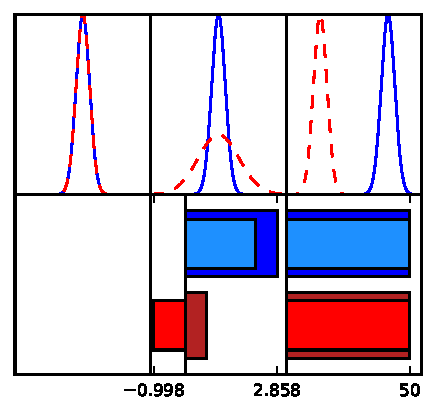
\includegraphics{../comparison/plots/surprise.pdf}
        \caption{The information gain from one distribution given a second distribution.
                 The top row shows the distributions, $P_1(x)$ in blue and $P_2(x)$ in red-dashed lines.
                 The bottom row shows the information gain.
                 The blue bars are obtained when $P_1(x)$ is updated by $P_2(x)$ and the red bars are obtained when $P_2(x)$ updates $P_1(x)$.
                 The darker bars are the relative entropy $D(P_1||P_2)$ or $D(P_2||P_1)$ in blue and red.
                 The lighter bars are the surprise $S$.}
        \label{fig:surprise}
    \end{figure}
    \noindent Since, in the first column, the two distributions are equal then the relative entropy is zero.
    This is expected so $\langle D\rangle = 0$ and thus $S = 0$.
    The second column is more interesting.
    When updating $P_1(x)$ using $P_2(x)$ (blue bars) there is an information gain because more of the parameter space is available.
    The expected relative entropy is small though since less about the parameters is known after this update.
    Finding the difference means that there is large amount of surprise.
    This amount of surprise can be quantified as a $p$-value in comparison to $\langle D\rangle$.
    A positive value of $S$ means that the distributions are more different than expected.
    On the other hand, updating $P_2(x)$ with $P_1(x)$ (as for the red bars) the information gain is slightly positive, but there is expected to be a large amount of information gain.
    This is because a large amount of information about the value of parameters is obtained by tightening the constraints.
    The surprise is therefore negative, this shows that the constraints are actually \emph{more consistent} than expected.
    The final column shows that the information gain obtained by updating $P_1(x)$ with $P_2(x)$ or vice versa is very large, but there is no \emph{expected} gain since the whole parameter space changes.
    Therefore the entirety of the information gain is due to surprise. 
    Comparing this large value of $S$ to $\langle D\rangle = 0$ gives a very small $p$-value, showing that the tension is high.
    The equivalent test in two dimensions can be found in Fig.~\ref{fig:surprise_2D}.
    \begin{figure}
        \centering
        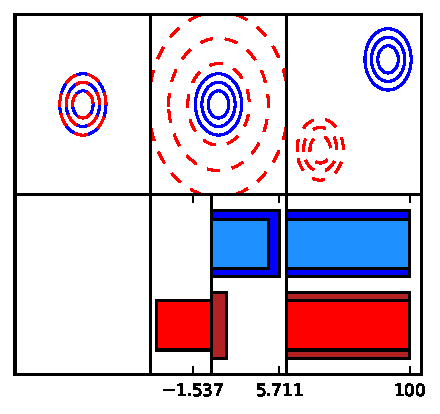
\includegraphics{../comparison/plots/surprise_2D.pdf}
        \caption{The information gain from one distribution given a second distribution in two dimensions.
                 The top row shows the distributions, $P_1(x)$ in blue and $P_2({\bf x})$ in red-dashed 1, 2 and 3$\sigma$ contours.
                 The bottom row shows the information gain.
                 The blue bars are obtained when $P_1({\bf x})$ is updated by $P_2({\bf x})$ and the red bars are obtained when $P_2({\bf x})$ updates $P_1({\bf x})$.
                 The darker bars are the relative entropy $D(P_1||P_2)$ or $D(P_2||P_1)$ in blue and red.
                 The lighter bars are the surprise $S$.}
        \label{fig:surprise_2D}
    \end{figure}
    \noindent As can be seen, the results are identical in meaning, if not in value.
    There is no information gain from two identical distributions.
    A wide distribution updating a narrow distribution causes a surprise driven information gain and a narrow distribution updating a wide distribution causes a small gain with negative surprise.
    Finally, two disparate distribution causes large information gain which is completely derived from surprise.
    \\
    \\
    Interestingly in Fig.~\ref{fig:surprise_2} there is a difference between the results in one dimension and two dimensions.
    The first column shows, as expected, that a shift in the mean of one of the distributions provides an information gain.
    Some of this comes from surprise, but most of this is expected as the shift is only small.
    Information is gained since some parameter space is ruled out, providing more knowledge on the parameter, but the parameter space has also widened due to the shift providing more available room for the parameter.
    In the middle column (the equivalent of Figs.~\ref{fig:2D_2} and~\ref{fig:under_2D}) though, the shift has provided information gain, but this is less than expected.
    The parameters are in closer agreement than would be expected due to this update.
    By moving the second distribution very slightly further from the first this reverts to similar behaviour to the left-hand column as can be seen in the right-hand column.
    This sensitive behaviour changes the interpretation of the results greatly for little change in the distributions.
    The difference between a distribution in a great amount of tension and a distribution in virtually no tension is extremely small.
    \begin{figure}
        \centering
        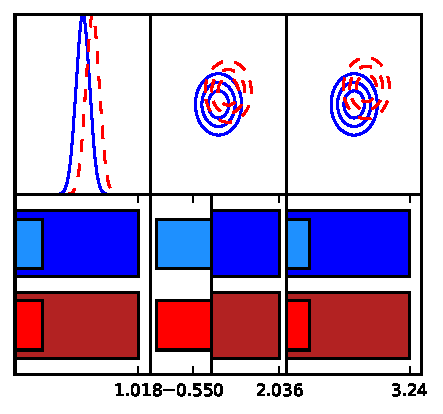
\includegraphics{../comparison/plots/surprise_2.pdf}
        \caption{The information gain from one distribution given a second distribution in two dimensions.
                 The top row shows the distributions, $P_1(x)$ in blue and $P_2({\bf x})$ in red-dashed lines in the first column and 1, 2 and 3$\sigma$ contours in the last two.
                 The bottom row shows the information gain.
                 The blue bars are obtained when $P_1({\bf x})$ is updated by $P_2({\bf x})$ and the red bars are obtained when $P_2({\bf x})$ updates $P_1({\bf x})$.
                 The darker bars are the relative entropy $D(P_1||P_2)$ or $D(P_2||P_1)$ in blue and red.
                 The lighter bars are the surprise $S$.}
        \label{fig:surprise_2}
    \end{figure}
    \noindent Finally for this method, the non-Gaussian case can be considered and is found in Fig.~\ref{fig:surprise_skew}.
    This again is exactly as expected.
    $P_1(x)$ and $P_1({\bf x})$ in the left and right subplots respectively are narrower than $P_2(x)$ and $P_2({\bf x})$ and so there is a large amount of surprise driven information gain due to updating $P_1(x)$ or $P_1({\bf x})$ using $P_2(x)$ or $P_2({\bf x})$.
    On the other hand, there is slightly less surprise when updating $P_2(x)$ or $P_2({\rm x})$ using $P_1(x)$ or $P_1({\bf x})$.
    Although the relative entropy comes mostly from surprise, there is some expected relative entropy coming from the overlapping regions of the distributions.
    \\
    \\
    This method is somewhat useful quantifying information gains and comparing this to what is expected.
        \begin{figure}
        \centering
        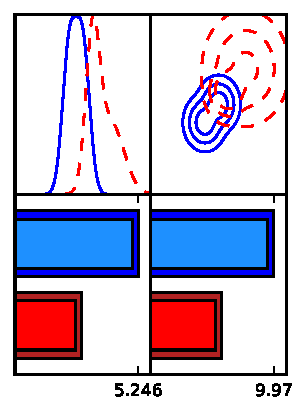
\includegraphics{../comparison/plots/surprise_skew.pdf}
        \caption{The information gain from one distribution given a second distribution in two dimensions.
                 The top row shows the distributions, $P_1(x)$ in blue and $P_2({\bf x})$ in red-dashed lines on the left and 1, 2 and 3$\sigma$ contours on the right.
                 The bottom row shows the information gain.
                 The blue bars are obtained when $P_1({\bf x})$ is updated by $P_2({\bf x})$ and the red bars are obtained when $P_2({\bf x})$ updates $P_1({\bf x})$.
                 The darker bars are the relative entropy $D(P_1||P_2)$ or $D(P_2||P_1)$ in blue and red.
                 The lighter bars are the surprise $S$.}
        \label{fig:surprise_skew}
    \end{figure}
    \noindent It does depend on choosing one data set to update another rather than stating how similar the two distributions are independent of each other.
    Also it seems very sensitive to small changes in distributions, as in the middle column of Fig.~\ref{fig:surprise_2}.
    Due to the interpretation of the results differing wildly by such a tiny change, care must be taken when carrying out the analysis.
    \\
    \\
    Other measures generally involve comparisons of Bayesian evidences.
    The most simple and commonly used was introduced in \cite{Marshall:2004zd}.
    This is given by
    \begin{equation}
        R = \frac{p(D_1, D_2)}{p(D_1)p(D_2)},
    \end{equation}
    where $p(D)$ is the evidence given data $D$,
    \begin{equation}
        p(D) = \int dx P_D(x)p(x),
    \end{equation}
    with $p(x)$ the prior on the parameter $x$ and 
    \begin{equation}
        p(D_1, D_2) = \int dx P_{1}(x)P_2(x)p(x).
    \end{equation}
    $R$ is therefore the ratio of the evidence given both data sets to the evidence of each data set.
    The prior assumptions of the parameter must be known and understood to calculate this result.
    Using $\log R$ the results can be interpreted on the Jeffery's scale with $\log R>0$ indicating agreement and $\log R<0$ indicating disagreement to some degree.
    The results are given in Table.~\ref{tab:R}.
    \begin{table}
        \centering
        \begin{tabular}{l|ccccc}
              & I & II & III & IV & V \\ \hline\hline
           1D & 1.730 & 0.926 & -23.270 & 1.221 & 0.120 \\
           2D & 3.460 & 1.851 & -46.540 & 2.442 & 1.108
        \end{tabular}
        \caption{Values of $\log R$ for each of the distribution comparisons. I, II and III refer to the distributions in each of the columns of Fig.~\ref{fig:bhattacharrya}, or Fig.~\ref{fig:2D} in the two dimensional case, respectively. IV describes the distributions with the shifted means such as in Fig.~\ref{fig:bhattacharrya_2} or Fig.~\ref{fig:2D_2}. V refers to the non-Gaussian distributions of Fig.~\ref{fig:skew} and Fig.~\ref{fig:skew_2D}.}
        \label{tab:R}
    \end{table}
    \noindent These results follow the general scheme of each of the other methods discussed earlier.
    More similar distributions score more highly whilst those in complete disagreement are negative (severely so, as shown here).
    This, as for the $BC$ and $OVL$ methods, suffers from confusing differences and variances.
    The numbers from $\log R$ are very dependent on the choice of priors.
    The trend stays the same, but the severity at which distributions disagree can change by quite a lot, whereas well fitting distributions can appear to fit slightly worse than they do under change in choice of prior.
    \\
    \\
    Similarly, another measure used in~\cite{Verde:2013wza} shifts one distribution (in a somewhat similar way to the $C$ method) so that the maxima of the two distributions coincide and then finds the ratio to the joint probability distribution
    \begin{equation}
        T = \frac{p(D_1,D_2)_{\rm shifted}}{p(D_1,D_2)}.
    \end{equation}
    $\log T$ can be used to quantify tension between datasets.
    Identical distributions have $\log T=0$ and $\log T>0$ indicates deviations from similarity.
    The results from each of the distributions are given in Table.~\ref{tab:T}.
        \begin{table}
        \centering
        \begin{tabular}{l|ccccc}
              & I & II & III & IV & V \\ \hline\hline
           1D & 0.000 & 0.000 & 25.000 & 0.509 & 1.110 \\
           2D & 0.000 & 0.000 & 50.000 & 1.018 & 1.505
        \end{tabular}
        \caption{Values of $\log T$ for each of the distribution comparisons. I, II and III refer to the distributions in each of the columns of Fig.~\ref{fig:bhattacharrya}, or Fig.~\ref{fig:2D} in the two dimensional case, respectively. IV describes the distributions with the shifted means such as in Fig.~\ref{fig:bhattacharrya_2} or Fig.~\ref{fig:2D_2}. V refers to the non-Gaussian distributions of Fig.~\ref{fig:skew} and Fig.~\ref{fig:skew_2D}.}
        \label{tab:T}
    \end{table}
    \noindent In Col.~II it can be seen that, like with the $C$ method, there is no punishment for widening the distribution and hence $\log T=0$ in both the one dimensional and two dimensional cases. 
    The disparate distributions have extremely large $\log T$ values showing that they disagree.
    The shifted mean and non-Gaussian results are greater than zero and indicate some difference in the data.
    Interpreting these numbers as an amount of deviation is difficult, in a similar way to $BC$, $OVL$ and $\log R$ these numbers do not directly map to a statistical significance or a $p$-value, although there is a vague description of meaning for the Jeffrey's scale for $\log R$.
    The values of $\log T$ can be expected to be twice as large when the dimensionality of the problem increases by two.
    This can either be corrected or taken into consideration when interpreting the result.
    \\
    \\
    Even though there are many ways to quantify the amount of tension or similarity or even information gain from two distributions, stating these results as a definitive value should come with a warning label.
    Every method has its drawbacks.
    For the Bhattacharrya distance this is the dependence on variance and the uncertainty in interpreting what the value of $0<BC<1$ means.
    For the overlap coefficient there is even greater variance dependence and again there is an issue with what the meaning of $0<OVL<1$.
    The method used in~\cite{Battye:2014qga} is more robust in some ways.
    For example, there is no variance dependence and the value of $C$ can be interpreted directly as a statistical significance.
    The problem here is why choose the integral defined by the isocontour of the difference vector at zero?
    This is fairly arbitrary and could be set to any other value.
    As a measure which seems to quantify differences well this shouldn't matter, apart from for ones own sanity.
    As stands, choosing this value to define the integral can be looked at from the opposite perspective.
    Integrating the probability distribution of the difference vector from the maximum (or maxima) to lower values until it contains $y=0 $ or ${\bf y}=0$ gives the amount of samples away from zero. 
    If 68\% of the samples are away from zero then the distributions disagree at the $1\sigma$ level.
    Another problem here is dealing with unusual non-Gaussian probability distribution functions.
    This is connected quite closely to the choice of integration contour.
    Perhaps a better way would be to find the distance from zero of the mean of the difference vector which could then be used a single measure.
    This would bring about its own problems, and probably still not work very well with non-Gaussian data.
    For $\Lambda$CDM cosmological parameters this probably won't matter too much as they are fairly Gaussian, no matter what data is constraining the values.
    The comparison of $I_1$ and $I_2$ has the greatest interpretive usefulness.
    The problem with this method arises because two numbers are now being used and the integration limits are arbitrary once again.
    This method seems the most robust of the different procedures described here.
    The \emph{surprise} method of~\cite{Seehars:2014ora} also works quite well, has two numbers which need to be interpreted, but unlike the $I_1$ and $I_2$ method is very sensitive to slight changes which can rapidly change the interpretation.
    Finally, the~\cite{Marshall:2004zd} and~\cite{Verde:2013wza} methods work to some extent.
    The first one suffers the same issues as the Bhattacharrya distance and the overlap coefficient but can be interpreted on the Jeffery's scale.
    The second is more robust the sense there is no dependence on the variance of otherwise identical distributions, but it is difficult to understand the meaning of $\log T$ apart from $\log T=0$ for identical distributions and then larger numbers represent distributions which disagree to a larger and larger extent.
    \\
    \\
    In other words, statistics is hard!

\bibliography{tension}

\end{document}
